\documentclass{article}
\usepackage{natbib}
\usepackage{graphicx}
\usepackage[english]{babel}
\usepackage[utf8]{inputenc}
\usepackage{url}
\usepackage{fancyhdr}
\pagestyle{fancy}
\fancyhf{}
\rhead{CSI 5387 Data Mining and Concept Learning}
\lhead{University of Ottawa}
\rfoot{Page \thepage}

\begin{document}

\begin{center}
    \textbf{\huge{CSI\_5387\_Assignment\_1}}
\end{center}

\textbf{Student Name: Lingfeng Zhang}

\textbf{Student Number: 300134245}

\smallskip

\hline

\bigskip

\textbf{Part A}

\bigskip

\textbf{1)a}

$X = \{1,1,1,1\}$

$Y = \{2,2,2,2\}$

Manhattan distance is:

$|1-2| + |1-2| + |1-2| + |1-2| = 4$

Euclidean distance is:

$\sqrt[2]{(1-2)^2 + (1-2)^2 + (1-2)^2 + (1-2)^2} = 2$

Supreme distance is:

$|1-2| = 1$

\bigskip

\textbf{1)b}

X = \{0101010001\}

Y = \{0100011000\}

$cosine = \frac{X\cdot Y}{|X||Y|} = \frac{2}{2\times \sqrt{3}} \approx 0.58$

Contingency table:

\begin{center}
\begin{tabular}{c c c c c}
&X\\ 
Y & & 1 & 0 & sum\\ 
 &1 & 2 & 2 & 4\\  
 &0 & 1 & 5 & 6\\
 &sum & 3 & 7 & 10
\end{tabular}
\end{center}

$Jaccard Coefficient = \frac{2}{2+2+1} = 0.4$

\bigskip

\textbf{2)a}

In this question, python statistic library is used to calculate mean, median, variance, standard deviation and the results are shown in below.

\begin{center}
\begin{tabular}{c c c}
&age &BMI\\ 
mean &36.20 & 32.32\\
median &32.00 &30.55\\
variance &195.64 &53.26\\
standard deviation &13.99 &7.30
\end{tabular}
\end{center}

\bigskip

\textbf{2)b}

In this question, the values about age and BMI are sorted first and then Q1, Q3, IQR and Range can be found easily. The results are shown in below.

\begin{center}
\begin{tabular}{c c c}
&age &BMI\\ 
Q1 &24 & 25.9\\
Q3 &45 &35.8\\
IQR &21 &9.9\\
Range &42 &24.7
\end{tabular}
\end{center}

\bigskip

\textbf{2)c}

In this question, python matplotlib.pyplot package is used and two boxplots are shown below. The information in boxplots is matched with values in question 2b.

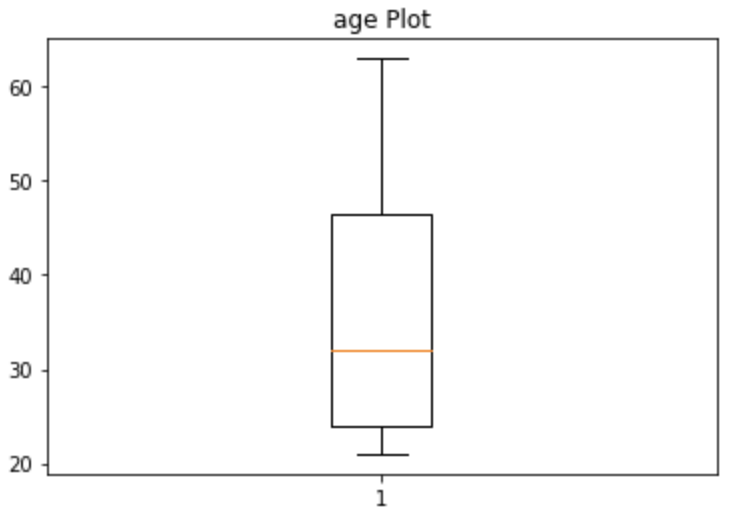
\includegraphics[scale=0.5]{age_boxplot.png}

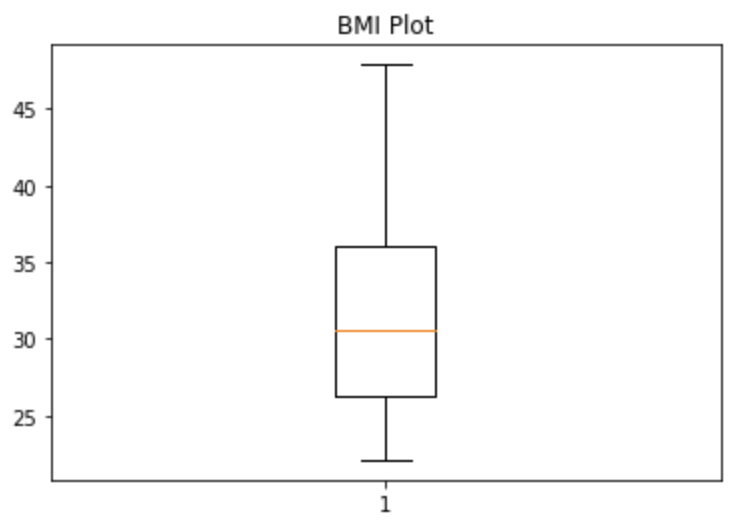
\includegraphics[scale=0.5]{BMI_boxplot.png}

\bigskip

\textbf{2)d}

The scatter plot is implemented by python matplotlib.pyplot.scatter() function and the plot is shown in below.

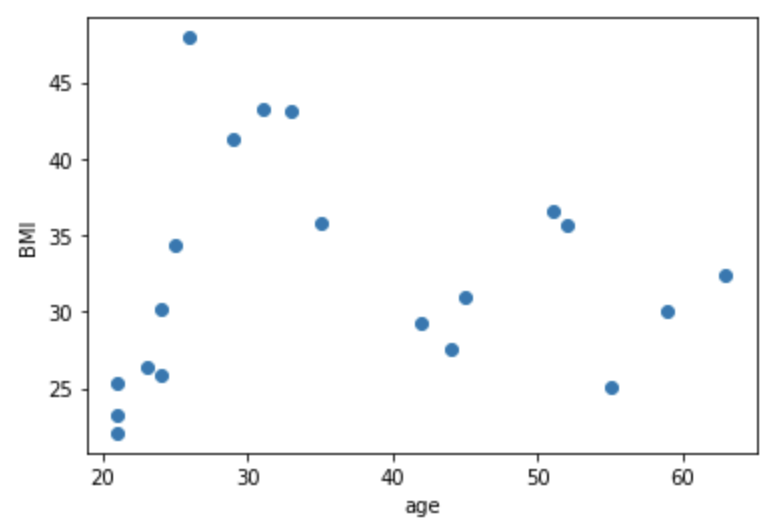
\includegraphics[scale=0.5]{scatter_plot.png}

The q-q plot is implemented by R qqplot() function and the plot is shown in below.

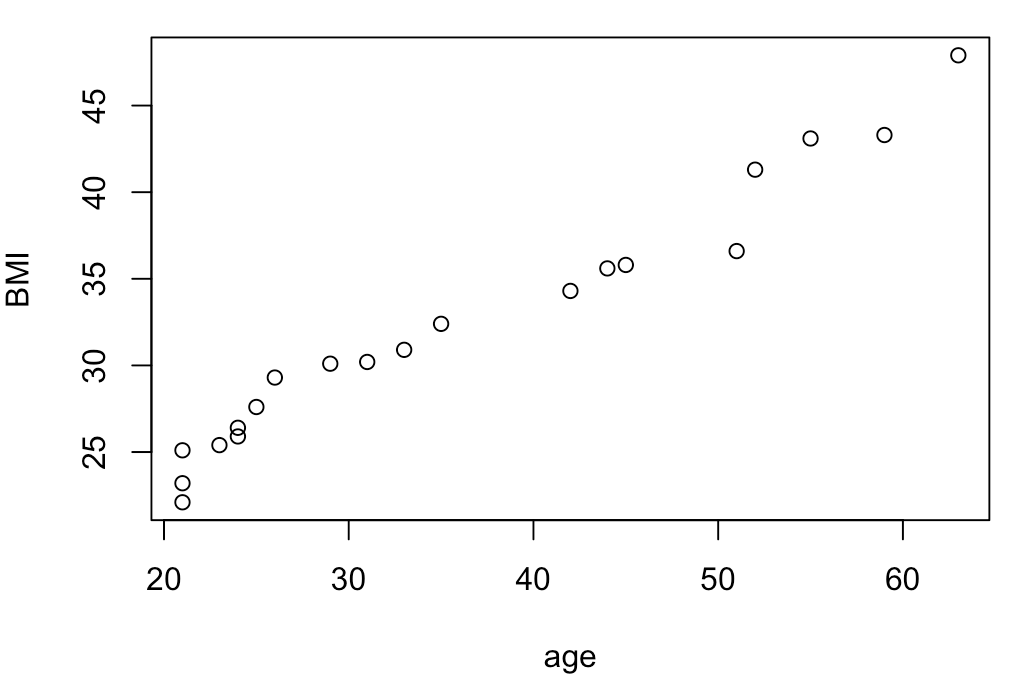
\includegraphics[scale=0.5]{qqplot.png}

\bigskip

\textbf{3)a}

According to the z-score function $z=\frac{x-\mu}{\sigma}$, two attributes are normalized as below results.


\begin{center}
\begin{tabular}{c | c}
age & BMI \\
\hline
-0.8948842494224685  &  -0.2987336962071037  \\
1.3790019581264261  &  -1.0156945671041535  \\
-0.08802140158253807  &  0.4885174561504412  \\
-0.748181913451572  &  2.189542267494423  \\
-0.9682354174079166  &  -0.8329398353068665  \\
1.1589484541700816  &  0.46040134356624374  \\
-0.8215330814370202  &  0.2776466117689559  \\
-0.8948842494224685  &  -0.9032301167673618  \\
1.9658113020100119  &  0.010543542219074666  \\
-0.38142607352433094  &  1.5428716780578677  \\
-0.2347237375534345  &  1.5147555654736704  \\
0.645490278271944  &  -0.20032730216241065  \\
1.672406630068219  &  -0.31279175249920244  \\
0.5721391102864959  &  -0.6642431598016779  \\
-0.5281284094952273  &  1.2617105522158873  \\
-1.1149377533788132  &  -1.2827976366540352  \\
-1.1149377533788132  &  -0.9735203982278569  \\
1.0855972861846335  &  0.6009819064872339  \\
0.42543677431559945  &  -0.4252562028359947  \\
-1.1149377533788132  &  -1.437436255867124
\end{tabular}
\end{center}

\bigskip

\textbf{3)b}

According to the formula of Pearson correlation coefficient:

\begin{center}
    $\rho_{X,Y} = \frac{E((X-\mu_X)(Y-\mu_Y))}{\rho_X \times \rho_Y}$
\end{center}

I use python scipy.stats.pearsonr() function to calculate this correlation value. The result is: 0.054.

\bigskip

\textbf{3)c}

Since the value of Pearson correlation coefficient in two attributes is positive, these two attributes are positively related.

\bigskip

\textbf{3)d}

According to the numpy.cov() function, the covariance matrix is given as below:

\begin{center}
\begin{tabular}{c c}
1.05263158 & 0.05649753 \\
0.05649753 & 1.05263158
\end{tabular}
\end{center}

So, the covariance number between attribute age and BMI is around 0.056.

\bigskip

\bigskip

\textbf{Part B}

In this part, Weka is used to analyze this dataset, which format is .arff.
\bigskip

\textbf{a.}

In Weka, principle component analysis and information gain attribute selection and correlation-based feature selection are used and I get different feature selection results.

As for principle component analysis, first 27 attributes are selected.

As for information gain attribute selection, all 29 attributes are selected.

As for correlation-based feature selection, only 5 attributes are selection, including sick(6), goitre(13), TSH(18), T3 measured(19), TT4(22).

\bigskip

Importance of feature selection:

1. Feature selection can reduce the dimensionality of the dataset and the machine learning models can be trained faster.

2. Feature selection can ignore irrelevant feature which will influence the accuracy of the training model becasue these features are noisy sometimes.

3. Feature selection can eliminate some redundant features which may affect the performance of some supervised learning models, such as Naive Bayes.

4. Feature selection can reduce the storage requirements.

5. Feature selection can reduce the probability of overfitting when training the model.

\bigskip

\textbf{b.}

In this case, I remove last 2 features according to the results of principle component analysis feature selection and use first 27 features to train the C4.5 decision tree.

In Weka, tree-based model J48 uses the principle of C4.5 decision tree and 10-fold cross validation is used without tree pruning.

To implement a decision tree, information gain should be calculated first and the attribute with the highest information gain should be selected and added into the tree structure. Then the dataset will be split according to various classes of last chosen attribute values. This process will continue recursively until reaching the boundary, like maximum tree depth or minimum node records. But this method of constructing the tree is likely to be overfitting. So tree pruning is a popular way to tackle with overfitting. Pruning reduces the complexity of the final decision tree. There are two common ways to handle tree pruning. The first one is reduced error pruning. This method is starting tree nodes and replacing each of them with the majority class. If the accuracy after replacement is not changed or higher, which shows that this node is unimportant and should be removed. Otherwise, this node can not be replaced. The another method of pruning is cost complexity pruning. The key idea of this method is calculating the accuracy of subtrees and see whether they have difference. If the accuracy of the subtree is same or better than the performance of the original tree, then this subtree can replace the original tree.

The C4.5 tree structure is shown below.

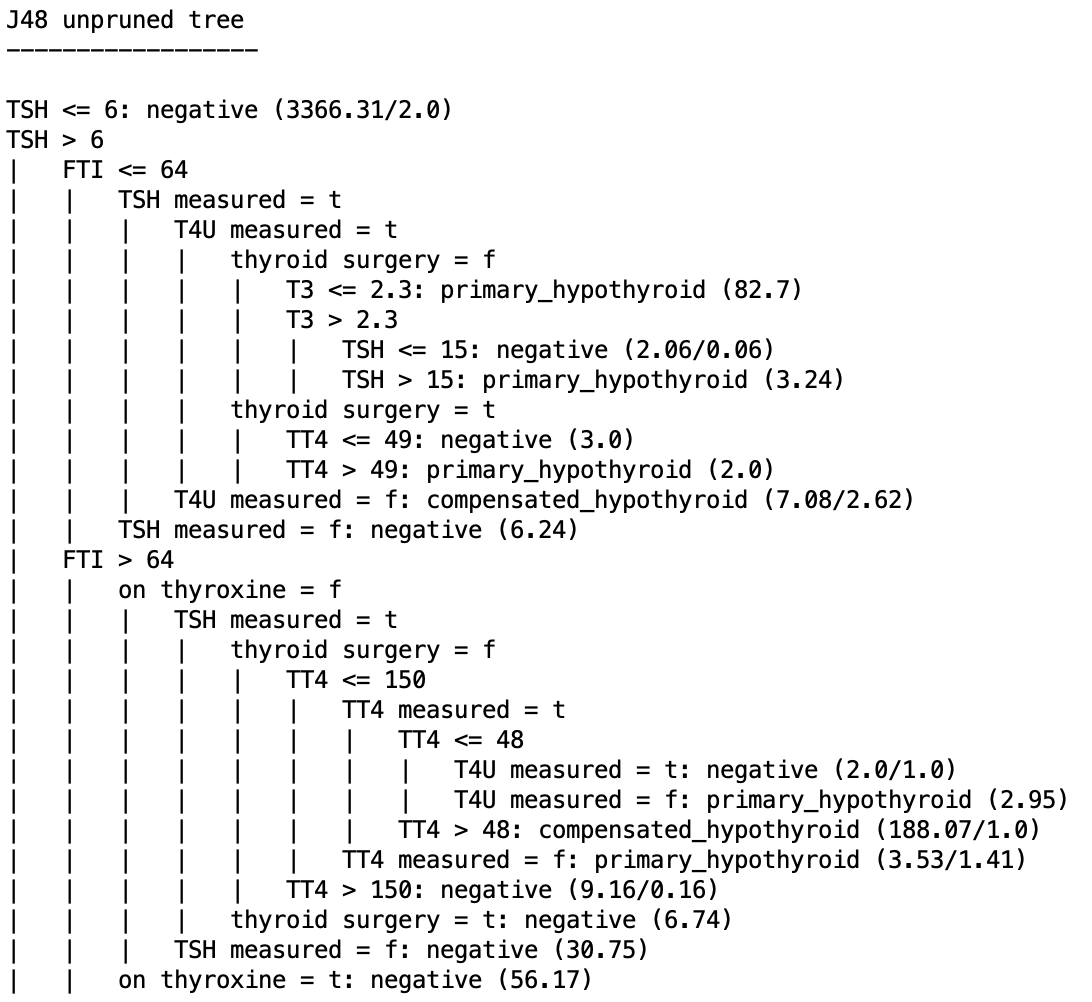
\includegraphics[scale=0.5]{tree_structure.png}

The C4.5 tree visualization is shown below.

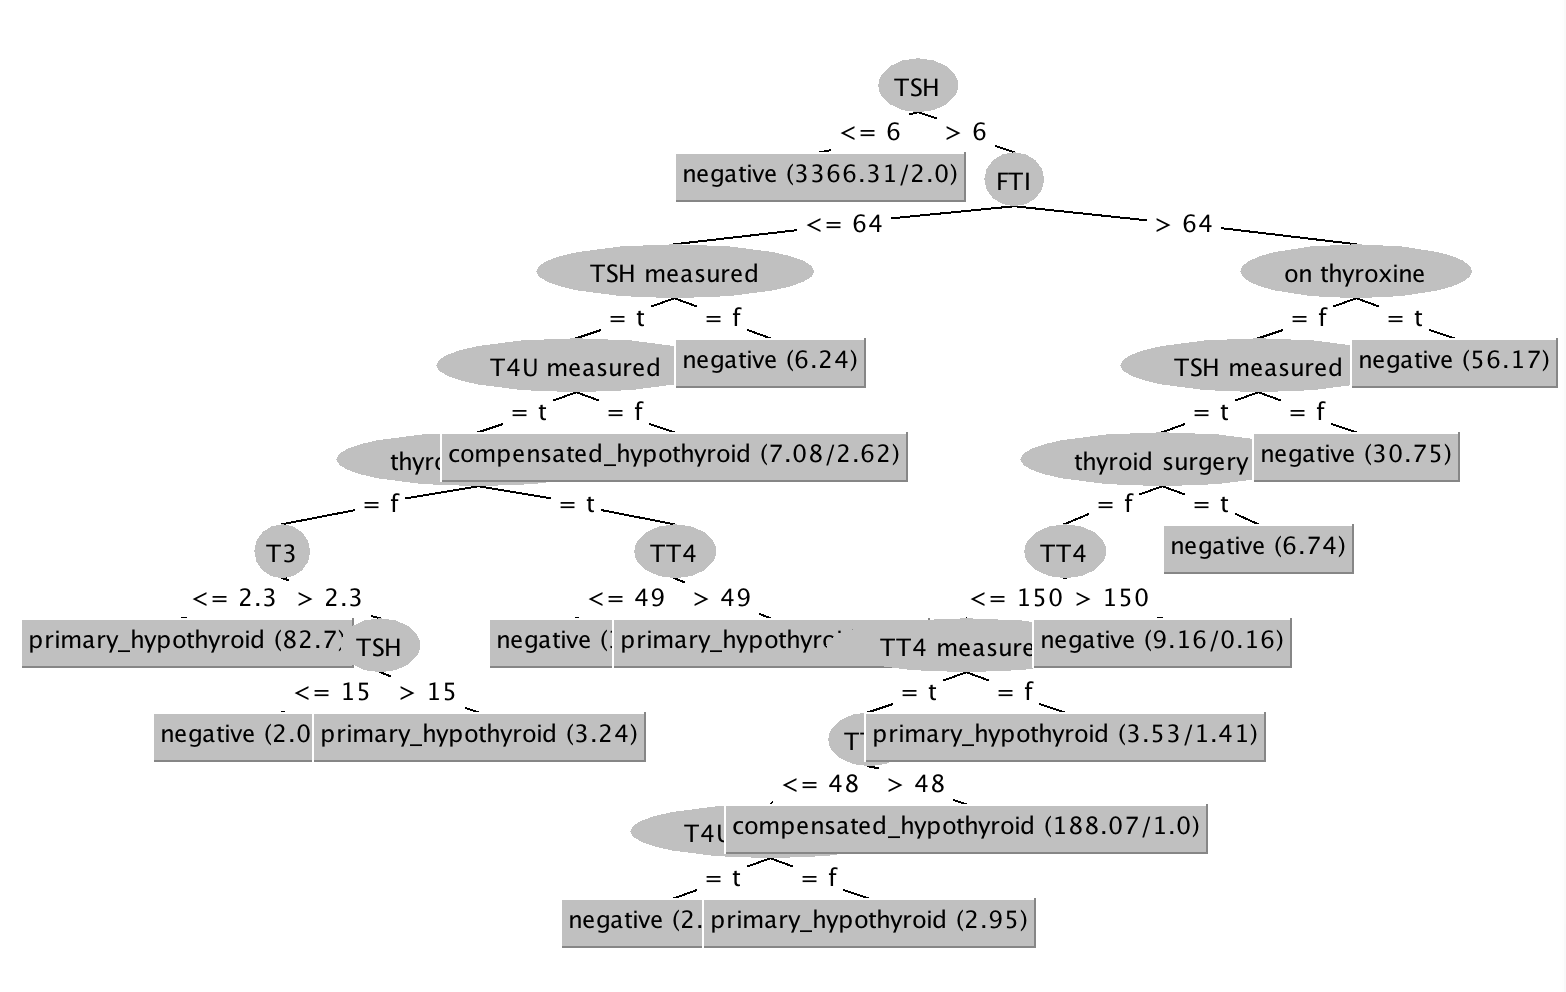
\includegraphics[scale=0.4]{tree_visualization.png}

As shown in this decision tree, when a new instance comes in, TSH is checked first, if TSH is less than or equal to 6, then this model predicts this instance as negative class. If TSH is larger than 6, then the second feature - FTI will be checked to compare with the number 64 and proceeding to the next branch, and so forth, until reach the leaf node in decision tree.

According to the generated decision tree structure, these rules can be extracted:

$1. IF(TSH<=6) \ THEN(class=negative)$

$2. IF(TSH>6 \ and \ FTI<=64 \ and \ TSH measured=f) \  THEN(class=negative)$

$3. IF(TSH>6 \ and \ FTI<=64 \ and \ TSH measured=t \ and \ T4U measured=f) \ THEN(class=compensated \ hypothyroid)$

$4. IF(TSH>6 \ and \ FTI<=64 \ and \ TSH measured=t \ and \ T4U measured=t \ and \ thyroid \ surgery=t \ and \ TT4<=49) \  THEN(class=negative)$

$5. IF(TSH>6 \ and \ FTI<=64 \ and \ TSH measured=t \ and \ T4U measured=t \ and \ thyroid surgery=t \ and \ TT4>49) \  THEN(class=primary \ hypothyroid)$

$6. IF(TSH>6 \ and \ FTI<=64 \ and \ TSH measured = t \ and \ T4U measured = t \ and \ thyroid surgery = f \ and \ T3<=2.3) THEN(class=primary \ hypothyroid)$

$7. IF(TSH>6 \ and \ FTI<=64 \ and \ TSH measured = t \ and \ T4U measured = t \ and \ thyroid surgery = f \ and \ T3>2.3 \ and \ TSH>15) \ THEN(class=primary \ hypothyroid)$

$8. IF(TSH>6 \ and \ FTI<=64 \ and \ TSH measured = t \ and \ T4U measured = t \ and \ thyroid surgery = f \ and \ T3>2.3 \ and \ TSH<=15) \ THEN(class=negative)$

$9. IF(TSH>6 \ and \ FTI>64 \ and \ on thyroxine=t) \  THEN(class=negative)$

$10. IF(TSH>6 \ and \ FTI>64 \ and \ on thyroxine=f \ and \ TSH measured=f) \ THEN(class=negative)$

$11. IF(TSH>6 \ and \ FTI>64 \ and \ on thyroxine=t \ and \ TSH measured=t \ and \ thyroid surgery=t) \ THEN(class=negative)$

$12. IF(TSH>6 \ and \ FTI>64 \ and \ on thyroxine=t \ and \ TSH measured=t \ and \ thyroid surgery=f \ and \ TT4>150) THEN(class=negative)$

$13. IF(TSH>6 \ and \ FTI>64 \ and \ on thyroxine=t \ and \ TSH measured=t \ and \ thyroid surgery=f \ and \ TT4<150 \ and \ TT4 measured=f) \ THEN(class=primary \ hypothyroid)$

$14. IF(TSH>6 \ and \ FTI>64 \ and \ on thyroxine=t \ and \ TSH measured=t \ and \ thyroid surgery=f \ and \ TT4<150 \ and \ TT4 measured=t \ and \ TT4>48) \ THEN(class=compensated \ hypothyroid)$

$15. IF(TSH>6 \ and \ FTI>64 \ and \ on thyroxine=t \ and \ TSH measured=t \ and \ thyroid surgery=f \ and \ TT4<150 \ and \ TT4 measured=t \ and \ TT4<=48 \ and \ T4U measure=f) \ THEN(class=primary \ hypothyroid)$

$16. IF(TSH>6 \ and \ FTI>64 \ and \ on thyroxine=t \ and \ TSH measured=t \ and \ thyroid surgery=f \ and \ TT4<150 \ and \ TT4 measured=t \ and \ TT4<=48 \ and \ T4U measure=t) THEN(class=negative)$

\bigskip

\textbf{c.}

C4.5 decision tree algorithm uses information gain as splitting method. Without pruning, this algorithm can achieve the accuracy at $99.5758\%$. The confusion matrix is shown below.

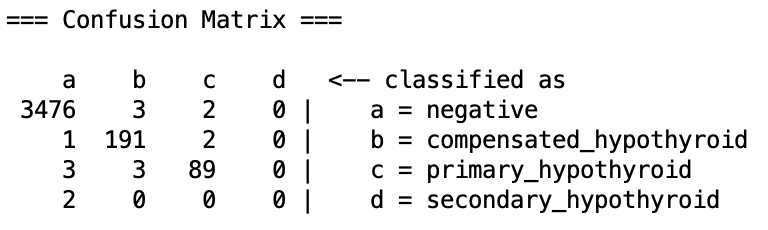
\includegraphics[scale=0.8]{j48_np_confusion_matrix.png}

After pruning, the accuracy still reaches at $99.5758\%$. Theoretically, tree pruning can improve the accuracy performance but in this case, there is probably no overfitting when training the model.

When using the dataset without the feature selection, tree pruning can improve the accuracy slightly because this model based on this dataset can perform well enough already.

Then, Hoeffding Trees with gini index and information gain are used but achieve lower accuracy scores, both $95.3075\%$. In addition,  Logistic model tree achieves relative low score, at $99.4433\%$.

In this case, C4.5 decision tree with pruning can achieve the highest accuracy score. In my view, according to the result of information gain feature selection, all attributes survive and we can know all attributes are useful. After principle component analyse dimensionality reduction, 27 features maintain. So, these selected features are more useful to build up the decision tree by using the information gain splitting method. This is probably the reason why C4.5 decision tree can achieve the best performance in this dataset.

Logistic model tree(LMT) just uses linear regression method to replace pruning method for avoiding overfitting. The basic idea and the tree splitting method of LMT are same as C4.5 decision tree. So the performance of LMT is close to that of C4.5.

Hoeffding tree is more suitable for large streaming dataset that can not be fit into the model once. Hoeffiding's inequality probably have a negative impact on the performance of Hoedffding tree because this dataset is not so large that can meet rules of the statistic.

\bigskip

\textbf{d.}

In Weka, choosing filter$\rightarrow$unsupervised$\rightarrow$attribute$\rightarrow$ReplaceMissingValues consequently, missing values can be replaced by the modes for non-numeric data or means for numeric data.

For example, without handing missing values, The information of attribute TSH is shown below.

\smallskip

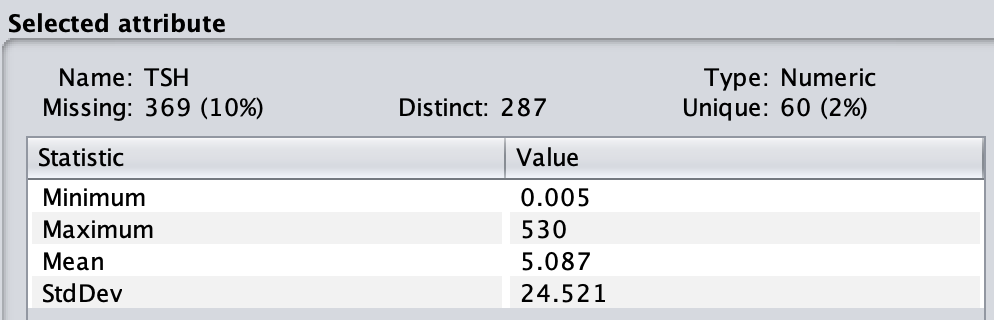
\includegraphics[scale=0.5]{tsh_origin.png}

After handing missing values by modes and means for each attribute, The information of attribute TSH is shown below. We can see $10\%$ missing values are handled and standard deviation has changed.

\smallskip

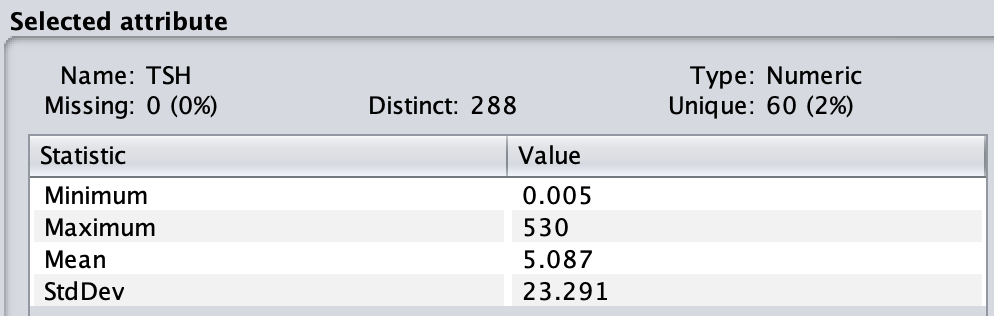
\includegraphics[scale=0.5]{tsh_missing.png}


\end{document}
